Sea $\mathbf{F}=\nabla\varphi$, con $\varphi(x,y)=xy+y^2$. Construya una parametrización por tramos de la trayectoria mostrada, calcule su trabajo directamente y compruébelo mediante el potencial.
\begingroup
\shorthandoff{>}
\begin{center}
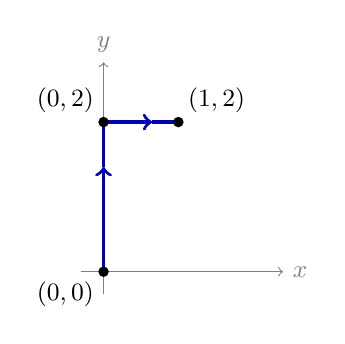
\begin{tikzpicture}[scale=.95,every node/.style={font=\small}]
    \draw[->,gray] (-.3,0)--(2.4,0) node[right] {$x$};
    \draw[->,gray] (0,-.3)--(0,2.8) node[above] {$y$};
    \draw[blue!75!black,very thick,->] (0,0)--(0,1.4);
    \draw[blue!75!black,very thick] (0,1.4)--(0,2);
    \draw[blue!75!black,very thick,->] (0,2)--(.65,2);
    \draw[blue!75!black,very thick] (.65,2)--(1,2);
    \fill (0,0) circle (2pt) node[below left] {$(0,0)$};
    \fill (0,2) circle (2pt) node[above left] {$(0,2)$};
    \fill (1,2) circle (2pt) node[above right] {$(1,2)$};
\end{tikzpicture}
\end{center}
\endgroup
